\documentclass[a4paper, 12pt, headings=standardclasses]{scrartcl}
\usepackage{titlesec}
\usepackage{graphicx}
\graphicspath{{figures/}}

\titlehead{\centering 
\includegraphics[width=8cm]{unilogo.pdf} \\ \Large{AG Kombinatorische Optimierung}}
\begin{document}
	\subject{\large{Bachelorarbeit}}
	\title{\LARGE{Genetic algorithms for the Traveling Salesman Problem (TSP)}}
	\author{Valeriya Sakharova}
	\date{June 12, 2019}
	
	\begin{titlepage}
		\maketitle
		\thispagestyle{empty}
	\end{titlepage}


\tableofcontents
\newpage

\section{Introduction}
\label{sec:introduction}
	 This bachelor thesis seeks to analyze and discuss the Traveling Salesman Problem(TSP), gives an overview to the existing ways how it can be solved with the help of Genetic Algorithms(GA), provides the implementation of them and discusses their effectiveness in comparison to each other. \par 
	 TSP is a problem, which looks for the shortest path through the given set of cities. Although it a theoretical problem, its is of great importance...Although the problem seems easy to be formulated, it is known to be NP-hard. It means that it cannot be solved exactly in polynomial time and therefore no exact algorithms can be used. The problem requires a compromise which is to be made between the quality of solutions and processing time. There exists a number of  approximation techniques, which can be applied to find a solution, which can be considered as good enough, taking into account the above mentioned issue. One of those techniques which are widely used in the literature is the so called genetic algorithms.\par
	 
	 TSPcan be solved either with exact orheuristic algorithm. Although it is easy to understand traveling salesman problem, but if thesizeisgettinglarger, its solutionusing exact algorithm will becomevery difficult. In term of quality and speed,solving the problemusing heuristicor meta-heuristicalgorithms is more feasible. Discovering a suboptimal solution with a sensible time or cost might be more beneficial rather than finding an optimal solution with time wasted. Various heuristic and meta-heuristic algorithms resulting in quick and good solutions have been devised.
	 
	 GA popular as they can be modified a lot...
	 Genetic algorithms are search and optimization algorithms which are based on natural selection and genetics. Each genetic algorithm includes several common steps, including selection, crossover, mutation, etc. But these steps can vary in their formulation. Therefore, the genetic algorithms can have plenty of modifications, which can influence its effectiveness. This purpose of this thesis is to give a detailed overview to the existing modifications of the genetic algorithms which are used to solve the TSP and to discuss their effectiveness. Another, not less important aim to be achieved in this thesis is to provide an implementation to these techniques, as the existing literature in this field does not generally provide the implementation and, moreover, does not specifies some general settings of the algorithms, which play a crucial issue in the effectiveness. \par
	 The structure of the thesis is as follows:\par
	 The Chapter 1 gives some theoretical background to the TSP and genetic algorithms. The Chapter 2 gives an overview to the existing crossover operators and discusses the main points in their implementation. \par The Chapter 3 provides the same overview concerning the mutation operators. The Chapter 4 discusses the problem of setting general parameters for genetic algorithms and provides the settings chosen for the aim of this thesis. The Chapter 5 makes a comparison study of different modifications of the genetic algorithms and discusses their effectiveness for solving Traveling Salesman Problem. At the end, the conclusion is given.
\section{General definitions}
\subsection{The TSP}
The traveling salesman problem (TSP) is a problem, where the shortest tour through the set of cities is to be found. Note that each city must be visited exactly once. The TSP is typically modeled as a directed, weighted graph, where each node represents a city. An edge between two nodes represents a path between the corresponding cities and he weight on the edge represents a distance between them. As a combinatorial optimization problem, it is often used to find the most efficient route for the given data between the given nodes. It is NP-hard, i.e. it cannot be solved exactly in polynomial time. \par

As the TSP is easily represented as a graph, we will use the terms of the graph theory in the following. Each city can be considered as a graph vertex. We say that there is an edge between two vertices, or cities, if these two cities are neighbours in the tour, whereas we will always have in mind that we work with a round tour, that is when we  write the tour 01234, we mean that there is an edge between the last and the first city. We call two vertices adjacent if they are connected by an edge. Two edges are called incident, if they share a vertex. Also, a vertex and an edge are called incident, if the vertex is one of the two vertices the edge connects.


\subsection{Genetic algorithms: general procedure}
This chapter gives an overview what a genetic algorithm is and which phases it contains.
Generally speaking, genetic algorithm is an approach for a randomized search, which simulates the natural selection process, where the fittest individuals are selected for reproduction, so that they can produce an offspring of the next generation. New individuals are created through the combination of genetic material from two parents, which is called crossover. This algorithm works on a population of chromosomes with the chosen finite size. The algorithm includes the calculation of the fitness value of each chromosome, selection of two parents to be crossed over and the application of mutation operators. The resulting offsprings, which correspond to the defined criteria, go to the next generation. The process repeats until the defined stop criteria are reached. Each phase of this algorithm is now discussed in detail.\par
\subsection{Genetic algorithms for the TSP}



\section{Representation types}
\subsection{Ordinal representation}
\subsection{Path representation}
\subsection{Random-key representation}
\subsection{Adjacency representation}
\subsection{Implementation details}


\section{Crossover operators}
\label{sec:crossover}
This chapter gives a general overview of the different variations of crossover operators. There exist a great number of different crossover operators which were elaborated for different very specific problems. However, we will concentrate  only on the operators which were used in the literature specifically for the TSP. \par
Crossover operators differ mainly in the way of preserving the order of the cities from the parent chromosomes. Some of them preserve the absolute order and the others preserve the relative order. They are discussed below, providing the examples of the corresponding approaches. At the end of this chapter, the general information  how these operators were implemented is given.

\subsection{Path representation crossovers}

Note that there exist more tours that represent the same round tour, where the start city is just different.
\subsubsection{Position-mapped crossover }
\label{subsec:pmx}
Position-mapped crossover (PMX) takes two indices, the substring between which goes from the first parent chromosome directly to the offspring at exactly the same position. The rest is filled with the cities from the second parent chromosome, preserving the positions. As a result, there can exist duplicates. To handle them, a mapping between two parents chromosomes at the indices between two cut points is made. According to this mapping, the duplicates in the created offspring are eliminated. \par

For instance, the first parent chromosome has the genes 051243, whereas the second parent chromosome consists of 132405. Let say, two cut points are 1 and 3. It means that the substring 512 goes to the offspring directly. As a result we get an offspring chromosome 1 512 05. To eliminate the duplicates we make a mapping between the elements between the cut points in the parents chromosomes, namely: 512 is mapped to 324, i.e. 5 is mapped to 3, 1 is mapped to 2 and 2 is mapped to 4.  As a result, we replace 1 with 2 in the offspring at the position 1 and get 251205. As we see, the replacement is not over as 2 is duplicated as well, therefore it will be replaced by 4 according to the mapping and we get 451205. Now we have to deal with the last 5 which can be replaced by 3. As a result we get an offspring 451203. If we switch the role of two parents chromosomes now, we can get the second offspring, which get the substring between cut points directly from the second parent chromosome and the rest is taken from the first parent chromosome.\par

Multiple replacements at the same position can occur if both parents have the same city in the part of the tour between the chosen cut points. For instance, the first parent is 051243 and the second parent is 125430. The chosen cut points are 1 and 3.  It means that 5 is mapped to 2, 1 is mapped to 5 and 2 is mapped to 4. The part between the chosen cut points from the first parent 512 goes directly to the offspring at the same positions, whereas the rest is taken from the second parent. As a result, we get the offspring 1 512 30. The city 1 is duplicated in the offspring, it means it will be replaced by another value according to the defined mapping, namely 1 is replaced by 5. Now the offspring consists of 5 512 30. However, the city 5 is duplicated as well and is replaced by 2, resulting the offspring 2 512 30. The city 2 is, however, duplicated as well, therefore an another replacement will be made. The city 2 is replaced by 4 according to the mapping. As the cities 3 and 0 are not duplicated, nothing will be done more. The resulting offspring is 4 512 30. 

\subsubsection{Cycle crossover} 
Cycle crossover(CX) looks for a cycle between two parent chromosomes. A cycle includes the subset of cities which takes the same subset of positions of the cities in both parent chromosomes. For instance, the first parent chromosome has the genes 0543162 and the second parent chromosomes has the genes 0435216. If both parents have the same cities at the same positions, so these cities go directly to the offspring at these positions. The subset of cities $\{3,4,5\}$ takes the same positions in both parents $\{1,2,3\}$, making a cycle 5-4-3-5. 
To find a cycle, we start from the index where the parent chromosomes differ from each other. It means that we ignore the city 0 which occupies the same position 0 in both parents, as it will not make any changes to the offspring. So we start with the index 1 where the city 5 is. Then we look for a city which stands at the same index in the second parent chromosome. In our case it is the city 4. Then we look for the index in the first parent chromosome where this city stands and using this index, namely the index 3, we find the city in the second parent chromosome which stands at this index as well, namely the city 3. Now we go to the first parent chromosome and see that the city 3 stands there at the index 4. In the second parent, the city 5 occupies the position 4 and we found a cycle 5-4-3-5. \par

The values of the found cycle is used to form the offspring. The cities are copied from the first parent chromosome to the offspring and occupy the same positions there. All the remaining positions are filled with the cities from the second parent chromosome at the exactly the same positions. As a result, the position of each city in the offspring is inherited from one of the parents and the resulting offspring is 0543216. So, each element comes from one parent together with its position.\par

Alternatively, to find the cycle we could start at random index and not at the beginning. Moreover, instead of just filling the remaining positions of the offspring with the cities from the second parent, we could use the cycles further, namely when all the possible cycles are found, they are alternately used from the parent chromosomes. Given the parent chromosomes 051463278 and 042315687. The first element is the same in both parents, so the city 0 goes directly to the offspring to the position 0. Here we have  three cycles, namely 5-4-3-5, 1-2-6-1, 7-8-7. So, at first, the subset of cities $\{3,4,5\}$,which corresponds to the first cycle, goes to the offspring at the positions from the first parent. Then the subset of cities $\{1,2,6\}$, which corresponds to the second cycle, goes to the offspring at the positions from the second parent. Finally, the subset $\{7,8\}$ goes to the offspring at the positions from the first parent again, resulting the offspring 052413678.


\subsubsection{Modified crossover}
This operator takes randomly an index, which corresponds to the cut point, which will be made on the first parent chromosome.
The cities before the cut point are taken from the first parent and go to the offspring at the same positions. The other indices of the offspring are filled with the cities from the second parent, where the search of the next city starts at the beginning of the second parent chromosome. As the duplicates may occur, to eliminate them, the next city goes from the second parent to the offspring only if this city has not been taken from the first parent chromosome yet. Otherwise, this city is ignored and the next city from the second parent goes to the offspring.\par

For instance, the first parent chromosome is 051243 and the second parent chromosome is 132045. Let the cut point be the index 2. Then, the cities which stand in the first parent before this cut point, namely 0 and 5, go directly to the offspring at the same positions. And now the cities from the second parent starting from the beginning of it are used. So, the city 1 goes to the offspring at the next free index, namely the index 2. So do the cities 3 and 2. The next city 0 has been already taken from the first parent chromosome, therefore it will be not used and the next city is taken into consideration, namely the city 4, which goes to the offspring at the last index. The last city 5 from the second parent has been already taken from the first parent, therefore we ignore it. The resulting offspring has the genes 051324.\par

\subsubsection{Order crossover}

Order crossover (OX) takes two indices, which correspond to 2 cut points. The part of the first parent chromosome between these indices, including the cities, which stands at them both, goes to the offspring directly at the exactly the same positions. The other positions will be filled with the cities from the second parent chromosome in the following way. Starting from the index, which stands just after the second cut point, the search for the next city in the second parent, which goes to the offspring at the same position, begins. If the city has been already used when the cities were copied from the first parent, the city in question will be ignored and the next city is considered. If the end of the second parent chromosome is reached during the search, the search continues at the beginning of it and can continue until the second cut point is reached. In the same way, the offspring is filled with the cities from the second parent, i.e. we start at the index just after the second cut point, fill the offspring till its end and then continue at the beginning of the offspring until the first cut point is reached.\par

For instance, the first parent chromosome is 150243 and the second parent chromosome is 132054 The chosen cut points are the indices 2 and 4. It means that the part of the first parent chromosome 024 goes directly to the offspring at the positions 2,3,4 correspondingly. Now the remaining part of the offspring will be filled. We start with the index after the second cut point and find the city 4 in the second parent chromosome. As this value has been already taken from the first parent chromosome, it cannot be used and the next city to be considered is the city 1 which stands at the index 0 in the second parent. This city has not been used yet, therefore it takes the position right after the second cut point, i.e. the position with the index 5, in the offspring. Now the end part of the offspring is full, therefore the next insertions continue at the beginning of the offspring chromosome, starting at the index 0. The next city in the second parent which is considered is the city 3. As it has not been used yet, it goes to the offspring at the position 0. The city 2 was already used, So was the city 0. Then the city 5 is inserted at the position 1 in the offspring. Now the second cut point in the parent chromosome is reached and the offspring is filled, therefore the crossover is over and the resulting offspring has the genes 350241.

\subsubsection{Linear order crossover}

Linear order crossover (LOX) works similar to the order crossover, which was discussed above. The difference is the remaining positions of the offspring are filled starting from the beginning of the offspring chromosome.  The search of the next candidate city in the second parent  starts at the beginning of the second parent chromosome and continues consequently till the end of it. 
Considering the example which was used above for order crossover with  the first parent chromosome 150243 and the second parent chromosome is 132054 and the indices 2 and 4, the offspring get the genes 024 at the positions 2,3,4 correspondingly. The remaining part of the offspring will be filled, starting with the first index 0. The candidate city for this position will be searched in the second parent at the position 0, where the city 1 will be found. As it has not been used in the offspring yet, it occupies the position 0 in the offspring. In the same way, the next city 3 from the second parent chromosome goes to the position 1 in the offspring. The positions 2 to 4 are already filled, therefore the next candidate from the second parent will go at the last index 5. And it will be the city 5, which can be taken into consideration in the second parent.Therefore, the resulting offspring has the genes 130245.
Note that this operator works exactly as the Order crossover does, if the cut interval is chosen at the end of the chromosome.


\subsubsection{Order-based crossover}
This operator randomly selects a subset of cities in the first parent chromosome and puts them into the offspring in the exactly the same order, in which these cities occur in the first parent, but at the positions, which these cities occupy in the second parent. Each remaining position in the offspring is filled with a city which occupies this position in the second parent. As a result, if the initial, randomly chosen subset of cities is two small, then the offspring is very similar to the second parent chromosome.\par

For instance, the the first parent chromosome is 051243 and the second parent chromosome is 132045. The chosen subset is $\{3,4,5\}$. These cities appear in the first parent chromosome in the order 5, 4, 3. This order must be preserved. In the second parent, they occupy the positions 1, 4 ,5. Therefore, these cities appear in the offspring in the defined order at the positions 1, 4, 5. The remaining positions are filled with the other cities from the second parent, preserving their positions. The resulting offspring has the genes 152043.

\subsubsection{Position-based crossover}
This operator takes randomly a subset of positions. The cities which occupy these positions in the first parent chromosome go directly to the offspring chromosome on the same positions. All the remaining positions of the offspring are filled with the cities from the second parent chromosome in the following way. Starting from the beginning of the second parent chromosome, the next city comes into the consideration. If it was already taken from the first parent, then the city is ignored and the next city on the consecutive position comes into question. It means that this operator preserves the absolute order of the cities which are taken from the first parent chromosome and the relative order of the cities, taken from the second parent chromosome.\par
For instance, the first parent chromosome is 051243 and the second parent chromosome is 132045. The set of chosen positions includes $\{1,3,4\}$. Cities 5, 2 and 4 occupy these  positions in the first parent and go at these positions in the offspring. Now the genes of the second parent chromosome are used. The city which occupy the starting position 0 in the second parent is the city 1. It has not been used yet, therefore, the city 1 goes to the offspring at the position 0.The next city in question is the city 3. It has not been used yet as well, therefore it occupies the next free position in the offspring, namely the position 2. The next two positions in the offspring are already filled. Therefore, the last position is filled with the city 0 from the second parent, which is the last city which has not been used yet.
So, the resulting offspring has the genes 153240.\par

\subsection{Adjacency representation crossovers}
The adjacency representation makes the changes in edges easier. The main aim of the crossover operators using this type of tour representation ist to preserve as many edges from the parent chromosomes as possible, as this type of representation allows to do it at best. The exception is the last edge, which is normally not inherited from the parents, as it is added to the final solution just to come to the first city to build the Hamilton cycle. \par

It is easy to understand this representation type, if one imagines an array, where each index number represents the city which has the edge with the city which stands in the array at this index. So it means, that the number of edges corresponds to the length of the array.\par

One can easily transform the tour in this representation into the path representation. As there is no a strict definition of the start city in this representation and as the choice of the first city will not influence the fitness value of the chromosome which can be made of this tour, one can start with the city number 0. It means that the next neighbor stands at the index 0 in the array. Then this city is considered to be a new index, where the next neighbor will be found. For instance, we have a tour in the array 1 4 0 2 3 in the adjacency representation. To get the path, we define the city 0 as the first city of the tour. We find the city 1 at the index 0 and it will be the next neighbor. At the index 1, stands the city number 4, which is added to the path. At the index 4, we find the city 3. Its neighbor is the city number 2, as it stands at the index 3. the city 0 is at the index 2 and we got the Hamilton cycle 0 1 4 3 2 0. (See Figure \ref{Adj_Path}).

\begin{figure}[!ht]
	\centering
	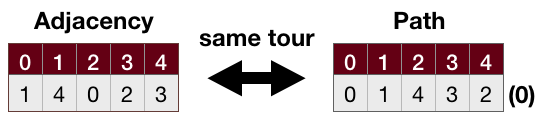
\includegraphics[width=0.5\textwidth]{Adj_Path}
	\caption{The same round tour in path and adjacency representation. }
	\label{Adj_Path}
\end{figure}

\subsubsection{Alternate edges crossover}
The alternate edges crossover (AE), which was described by Grefenstette et al. in \cite{grefenstette1985genetic}, alternately chooses the edges from parents. It includes the following steps:

\begin{enumerate}
	\item Choose two parent chromosomes.
	\item Choose randomly an edge from one of the parents as a starting point for the child tour.
	\item Choose the appropriate edge from the other parent and extend the tour.
	\item If the chosen edge introduces a cycle, choose a random edge, which does not introduce a cycle and extend the tour.
	\item Extend the tour further by choosing the edges alternatively from the parents until all the cities are included into the tour.	 
\end{enumerate}

For instance, we have the following parent tour: 123450 and 140532. Let assume, that the edge (0, 1) was randomly chosen from the first parent. It will be directly introduced in the child (See Figure \ref{alternate_edges_1}). The next edge (1, 4), which is incident to the city 1, will be taken from the second parent and put into the child tour. The next edge (4, 5) comes from the first parent. 

\begin{figure}[!ht]
	\centering
	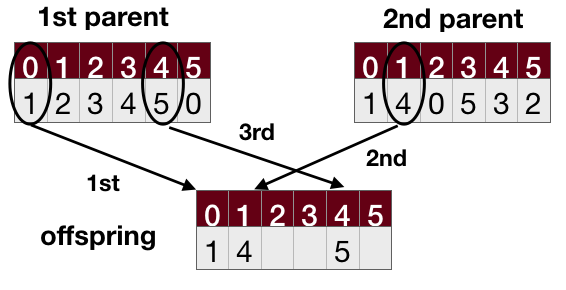
\includegraphics[width=0.5\textwidth]{alternate_edges_1}
	\caption{Alternate edges crossover: introducing the edges (0, 1), (1, 4), (4, 5).}
	\label{alternate_edges_1}
\end{figure}

The next two edges are (5, 2) and (2, 3) and extend the tour, as it shown in the Figure \ref{alternate_edges_2}.
The last edge is supposed to be taken from the second parent and it would be the edge (3, 5). 

\begin{figure}[!ht]
	\centering
	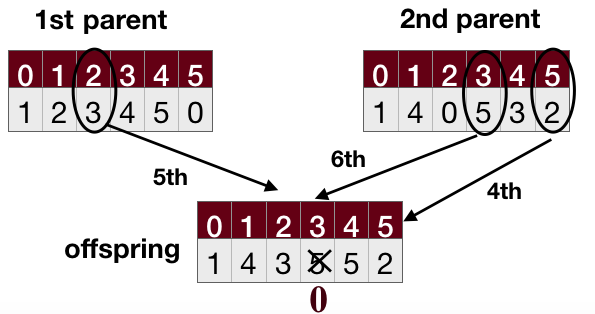
\includegraphics[width=0.5\textwidth]{alternate_edges_2}
	\caption{Alternate edges crossover: introducing the edges (5, 2), (2, 3).}
	\label{alternate_edges_2}
\end{figure}

However, it introduces a cycle and cannot be taken (See Figure \ref{alternate_edges_3}).
 
\begin{figure}[!ht]
	\centering
	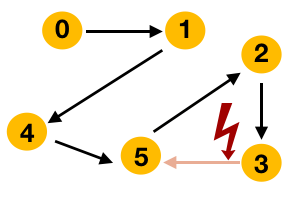
\includegraphics[width=0.3\textwidth]{alternate_edges_3}
	\caption{Alternate edges crossover: cycle in the tour after adding the edge (3, 5).}
	\label{alternate_edges_3}
\end{figure}

Instead, the last possible edge (3, 0) is chosen and finishes the tour. As this edge was the only possible edge to extend the tour, the random choice could not happen in this case. The resulting child tour is 143052. According to Grefenstette et. al \cite{2}, the results of this crossover was discouraging. Nevertheless, we implement this crossover operator as well and take a look at the results.

\subsubsection{Edge recombination crossover}
The edge recombination(ER) crossover uses a special data structure called 'edge map'. To build the edge map, for each city make a list of cities, which are the neighbors of this city either in the first parent or in the second parent chromosome. That is, for each city find all adjacent cities in both parents. \par

For instance, we have two parent chromosomes 02314 and 31420. The city 0 have the adjacent, or neighbor, cities 2, 3, 4 in both parents. The list for the city 1 includes 3, 4. The city 2 has the neighbors 0, 3, 4 and so on. (See Figure \ref{edge_map}.) 

\begin{figure}[!ht]
	\centering
	\includegraphics[width=0.5\textwidth]{edge_map}
	\caption{Initial state of the edge map for the parent chromosomes 02314 and 31420.}
	\label{edge_map}
\end{figure}

\begin{figure}[!ht]
	\centering
	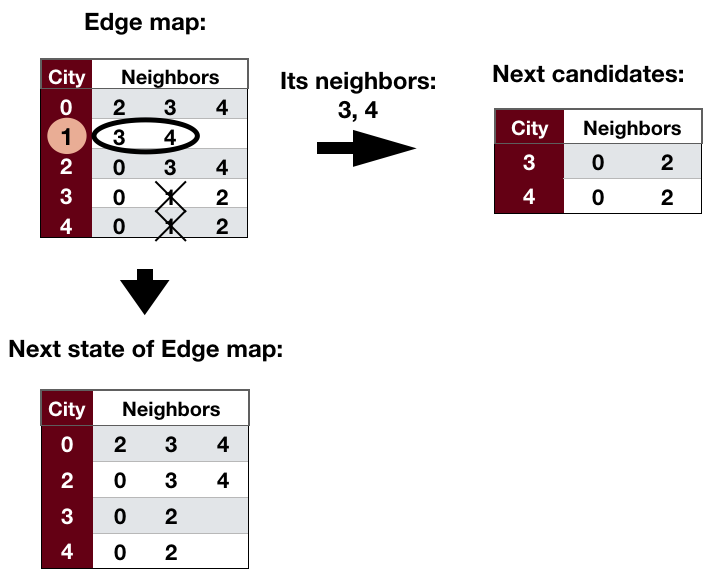
\includegraphics[width=0.5\textwidth]{Edge_map_after_city_chosen}
	\caption{IState of the edge map for the parent chromosomes 02314 and 31420 after choosing the city 1}
	\label{Edge_map_after_city_chosen}
\end{figure}

\begin{figure}[!ht]
	\centering
	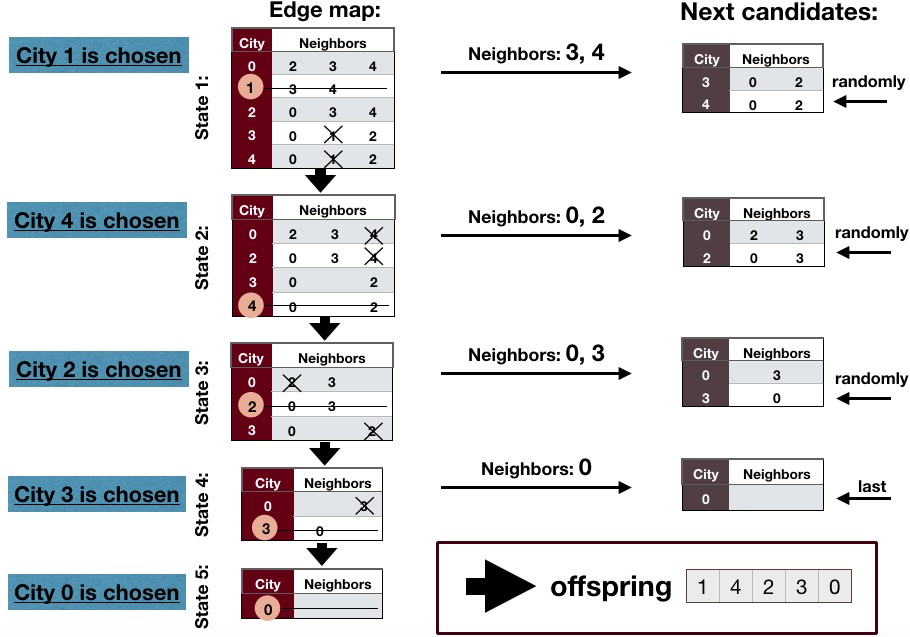
\includegraphics[width=\textwidth]{er}
	\caption{Edge recombination crossover.}
	\label{er}
\end{figure}

 That is, the edge map contains the list of edges that are incident to each city in the parent tours. This is the initial state of the edge map, because no cities have been included in the offspring yet. All the edges in the edge map are called "active", as they are available to continue the tour. Among these edges, the one will be chosen, which leads to the city with the minimal number of active edges. In other words, the city will be chosen, which list of neighbors is the smallest. If there are more than one candidate city, the choice is made randomly among them. The edge map will be update after each city selection, so that only active edges stay there.\par
 We will demonstrate how the edge recombination crossover works using the above mentioned parent chromosome and the constructed edge map on the Figure \ref{edge_map}.

 The city with the shortest list of neighbors is the city $1$. So, it will be selected and added to the tour. This city has the list of neighbors, including the cities $3$ and $4$. Therefore, these cities will be now considered as the next candidates to continue the tour and the used city $1$ will be deleted from the map (See Figure \ref{Edge_map_after_city_chosen}). In the Figure \ref{er}, it is shown, how the edge map transforms while doing this crossover. So, the next step is to compare  the candidates according to the length of their list of neighbors. The candidate with the shortest list will be chosen. If some candidates have the lists of neighbors of the equal length, as in our example the cities $3$ and $4$, then one of them will be taken randomly. Let assume, that the city $4$ was randomly chosen. It will be added to the tour and deleted from the edge map. As this city has the cities $0$ and $2$ as neighbors, they are the next candidates to continue the tour. Both cities have the same number of neighbors, there fore one of the them will be chosen randomly. Let assume, that the city $2$ was chosen and will be added to the tour. Its neighbors have the same length of the neighbors' list as well, therefore the city $3$ is assumed to be chosen randomly. This city continues the tour and its only neighbor, the city $0$, finishes the tour. The resulting tour is 14320.\par
 There is a modification of this type of crossover, where the edges which are common in both parents have the priority to be selected, even if they do not correspond to the city with the shortest list of neighbors.
 
\subsubsection{Heuristic crossover}
The heuristic crossover (HX) was introduces by Grefenstette et al. in \cite{grefenstette1985genetic} and \cite{grefenstette1987incorporating} for improving the effectiveness of the genetic algorithm for the TSP. As a rule, genetic algorithms are free from an exact domain information, what makes them widely used.  For better performance on a specific domain, the so called "hybrid" genetic algorithm can be introduced, where some domain-dependent information is used. So, the heuristic crossover, proposed by  by Grefenstette et al., considers the distances on the edges and looks for the shortest parental edge to an unvisited city. The HX algorithm includes the following steps:

\begin{enumerate}
	\item Choose two parent chromosomes.
	\item Choose randomly a city as a starting point for the child tour.
	\item Find the shortest edge, containing the chosen city, from both parents.
	\item If the shortest parental edge leads to a cycle in the current part tour,
	 choose randomly an edge, which does not introduce a cycle.
	 \item Go to the step $3$ and continue to extend the current part tour by choosing the shorter of the 4 edges in the parents which extend the tour, until all the cities are included into the tour.	 
\end{enumerate}

Note that Grefenstette et al. considers the asymmetric TSP, therefore only 2 edges are considered in the original algorithm. Although, we consider an assymetric TSP, we still implementing this variant, as ...  Moreover, there exist some modifications to this algorithm, one of which we include in the algorithm as well. So Liepins et al. \cite{liepins1987greedy} and Suh et al. \cite{suh1987incorporating} proposed the modification of the step $4$ as:
If the shortest parental edge leads to a cycle in the current part tour, choose the other parental edge. If it also introduces a cycle, then extend the tour with a random edge that does not introduce a cycle. 

For instance, we have two parent chromosomes 13420 and 14302. Let assume that the first edge was chosen at the index 0. As the 0th edge in the both parents is the same, so the offspring gets this edge, i.e. 1 goes at the index 0. Now 1 is the next index. The edge (1, 3) in the first parent has the distance 7, whereas the edge (1, 4) in the second parent has the distance 10 (see the distance table in Figure \ref{dist_table} ). 
 \begin{figure}[!ht]
	\centering
	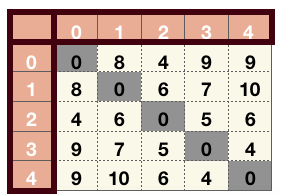
\includegraphics[width=0.3\textwidth]{dist_table}
	\caption{Distance table.}
	\label{dist_table}
\end{figure}

\begin{figure}[!ht]
	\centering
	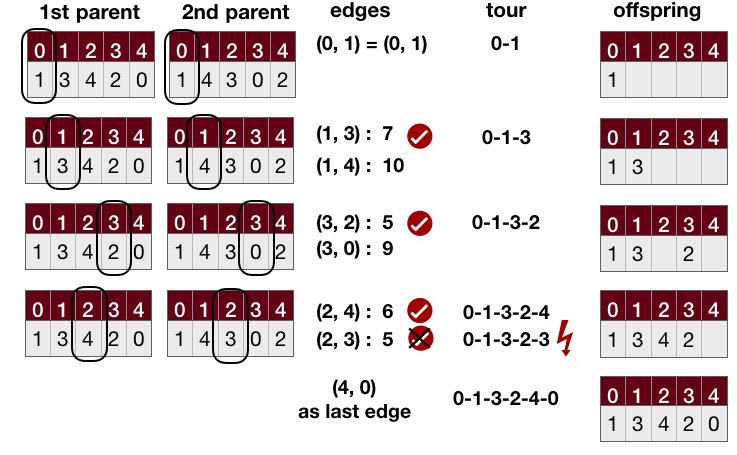
\includegraphics[width=\textwidth]{hX}
	\caption{Heuristic crossover for parent chromosomes 13420 and 14302.}
	\label{hX}
\end{figure}
Choosing the edge with the smallest distance, we choose the edge from the first parent and check, if it leads to a subcycle. The current tour of the offspring with this edge is 0-1-3. We do not have a subcycle here, therefore the edge (1, 3) goes to the offspring. The next index is 3. The edge (3, 2) in the first parent with its distance 5 wins against the edge (3, 0) in the second parent having the smaller distance 5 versus 9. The current tour of the offspring is 0-1-3-2. The next index 2 brings us to the edge (2, 4) in the first parent with the distance 6 and to the edge (2, 3) in the second parent with the distance 5. Therefore the edge (2, 3) wins but it introduces a sub cycle 0-1-(3-2-3). Therefore the other edge (2, 4) is taken, making the offspring 1342-. There is no choice for the last edge, because we need a Hamilton cycle. Therefore the offspring has the chromosome 13420, repeating the first parent (see the Figure \ref{hX}).
 
It is interesting to note, that this crossover tend to repeat one of the parents is the number of genes is small.

\subsection{Implementation details}
By implementing the different types of the crossover operators, they were classified according to the criteria how the cities are chosen from the parent chromosomes. According to this criteria they are divided into the operators, which use cut points and the ones which chose the subsets. Therefore, an abstract class Crossover was defined, from which the abstract classes CrossoverCycleSubset und CrossoverCutPoint inherit. Taking into consideration that there exist operators which use not only one cut point but two cut points, we get the continuation of the inheritance, where the abstract class CrossoverTwoCutPoints inherits from the abstract class CrossoverCutPoint. In the same way there is one more branch of inheritance in the other direction. The abstract class CrossoverRandomIndices inherits from the abstract class CrossoverCycleSubset.


\section{Mutation operators}
Mutation is one of the most important operators of the GA. It prevents the algorithm to stuck in a local minimum. It adds randomness in the evolutional process and can help to get genes, which were lost and cannot be reproduced otherwise. So, mutation diversifies the population.\par
Mutation operators for the TSP make random permutations of the cities and therefore, they can modifies the tour a lot. The mutation operators, which will be discussed below, will be applied only for the path representation. Applying them on the adjacency representation can ruin the round tour. For instance, let say the following tour in the path representation is 0, 1, 4, 3, 2, which corresponds to the tour in the adjacency representation 1, 4, 0, 2, 3. If we swap two cities 1 and 3, it results in the tour 0, 3, 4, 1, 2 in the path representation. The Hamilton cycle is still there.The adjacency representation looks like 3, 4, 0, 2, 1. The corresponding graph in the Figure \ref{mut_intro} illustrates that there exist two cycles and the Hamilton cycle was destroyed. \par

\begin{figure}[!ht]
	\centering
	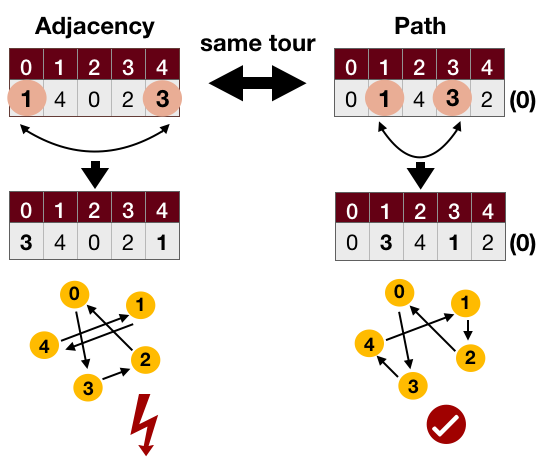
\includegraphics[width=5cm,height=5cm]{Mut_Intro}
	\caption{Swapping cities in adjacency and path representation.}
	\label{mut_intro}
\end{figure}

\subsection{Swap mutation}
This mutation operator \cite{potvin1996genetic} modifies the tour slightly, only exchanging the positions between of two cities. Given the chromosome 0,1,4,5,3,2 the swap mutation between the cities 4 and 3, which occupy the positions 2 and 4 accordingly, transforms the chromosome into 0,1,3,5,4,2(See Figure \ref{swap_mutation}).

\begin{figure}[!ht]
	\centering
	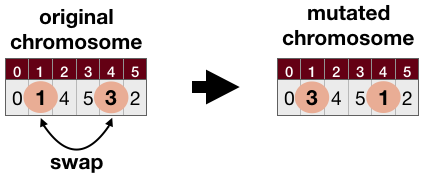
\includegraphics[width=0.4\textwidth]{swap_mutation}
	\caption{Swap mutation for the chromosome 0,1,4,5,3,2 with the swap for the cities 1 and 3.}
	\label{swap_mutation}
\end{figure}

\subsection{Scramble mutation}

This mutation operator \cite{potvin1996genetic} takes two indices, which define two cut points. The cities between and inclusive these cut points are randomly permuted. Given the chromosome 0,1,4,5,3,2 the scramble mutation for the cut points 1 and 4 can generate, for instance, the chromosome 0,3,5,1,4,2 (see Figure \ref{scramble_mutation}).

\begin{figure}[!ht]
	\centering
	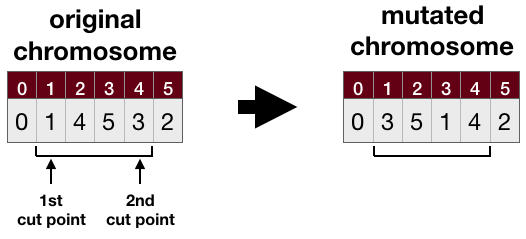
\includegraphics[width=0.4\textwidth]{scramble_mutation}
	\caption{Scramble mutation for the chromosome 0,1,4,5,3,2 with the cut points 1 and 4.}
	\label{scramble_mutation}
\end{figure}

\subsection{Shift mutation}

This mutation operator has two random components: a random city and a random integer. The chosen city will be shifted to the left or to the right, depending which shift is used. The chosen integer corresponds to the number of positions, at which the chosen city will be shifted. Given the chromosome 0,1,4,5,3,2. Let assume, that a random city is the city 1 and a random integer is 3. We will use the right shift. Therefore, the city 1 will be shifted to the right at 3 positions (see Figure \ref{shift_mutation}).

\begin{figure}[!ht]
	\centering
	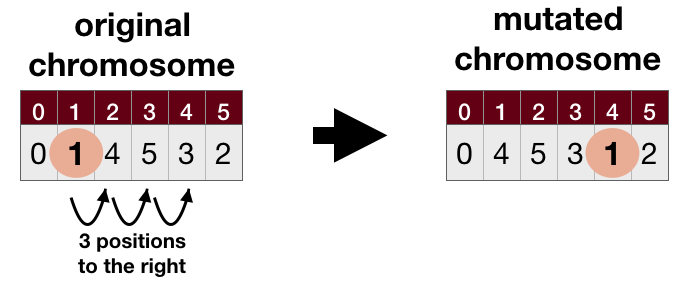
\includegraphics[width=0.4\textwidth]{shift_mutation}
	\caption{Right shift mutation for the chromosome 0,1,4,5,3,2 with a random city 1 and a random integer 3.}
	\label{shift_mutation}
\end{figure}

If the chosen integer is greater than the number of remaining steps to the right (or to the left, if the left shift is chosen), than the chromosome is assumed to be a torus and the shift begins from the corresponding another end of the chromosome. For instance, if a random integer was 5 in the example above, than the city 1 will be at the position 0 (see Figure \ref{shift_mutation_torus}).

\begin{figure}[!ht]
	\centering
	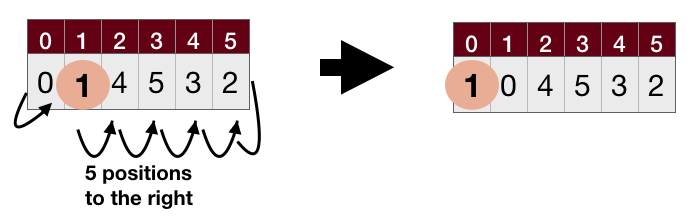
\includegraphics[width=0.4\textwidth]{shift_mutation_torus}
	\caption{Right shift mutation for the chromosome 0,1,4,5,3,2 with a random city 1 and a random integer 5.}
	\label{shift_mutation_torus}
\end{figure}

\subsection{Inversion mutation}

This mutation operator \cite{akay2013recent} takes two indices, which define two cut points. The cities within them(inclusively) are inverted. Given the chromosome 0,1,4,5,3,2 the inversion mutation for the cut points 1 and 4 generates the chromosome 0,3,5,4,1,2 (see Figure \ref{inversion_mutation}).

\begin{figure}[!ht]
	\centering
	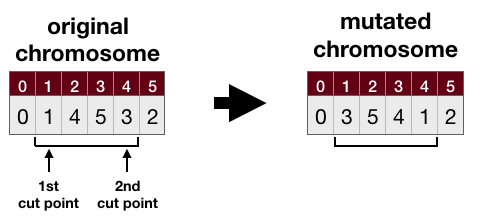
\includegraphics[width=0.4\textwidth]{inversion_mutation}
	\caption{Inversion mutation for the chromosome 0,1,4,5,3,2 and cut points 1 and 4.}
	\label{inversion_mutation}
\end{figure}

\subsection{Insertion mutation (2-opt exchange)}
This mutation operator \cite{akay2013recent} takes two indices, which define two cut points. The cities which occupy the positions between the first cut point(exclusively) and the second cut point(inclusively) are shifted one position to the left, i.e. back to the beginning. The city which occupied the index, which corresponds to the first cut point, now goes at the index, which corresponds to the second cut point, i.e. this stands after the set of shifted cities now. Given the chromosome 0,1,4,5,3,2 the insertion mutation for the cut points 1 and 4 generates the chromosome 0,4,5,3,1,2 (see figure \ref{insertion_mutation}).
It corresponds to a single 2-opt exchange...

\begin{figure}[!ht]
	\centering
	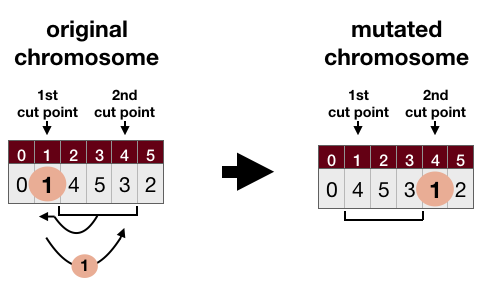
\includegraphics[width=0.4\textwidth]{insertion_mutation}
	\caption{Insertion mutation for the chromosome 0,1,4,5,3,2 and cut points 1 and 4.}
	\label{insertion_mutation}
\end{figure}

\subsection{3-opt exchange}

In 2-opt exchange we remove 2 links from the tour, this way obtaining 2 open segments, which we can manipulate and combine them to get a new tour. In 3-opt we remove 3 links, obtaining 3 segments to manipulate. This gives us eight combinations (including the tour identical with the initial one). These eight combinations include: 1 equivalent original tour,
3 cases which correspond to a single 2 -opt exchange, 3 cases which correspond to to two subsequent 2-opt exchanges and the last case, which is equivalent to three subsequent 2-opt moves. Therefore, we do not implement 3-opt exchange explicitly, as it will automatically happen while using 2-opt exchange subsequently (see figures \ref{toDo1} and \ref{toDo2} )

\begin{figure}[!ht]
	\centering
	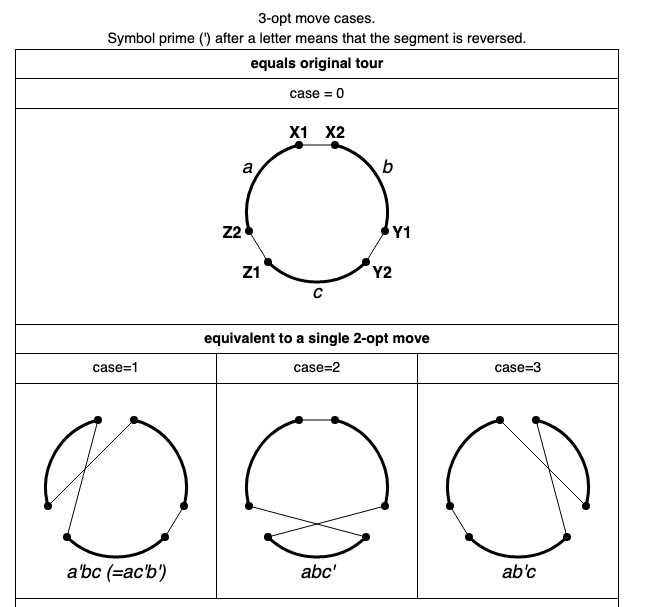
\includegraphics[width=0.4\textwidth]{toDo1}
	\caption{TODO1}
	\label{toDo1}
\end{figure}

\begin{figure}[!ht]
	\centering
	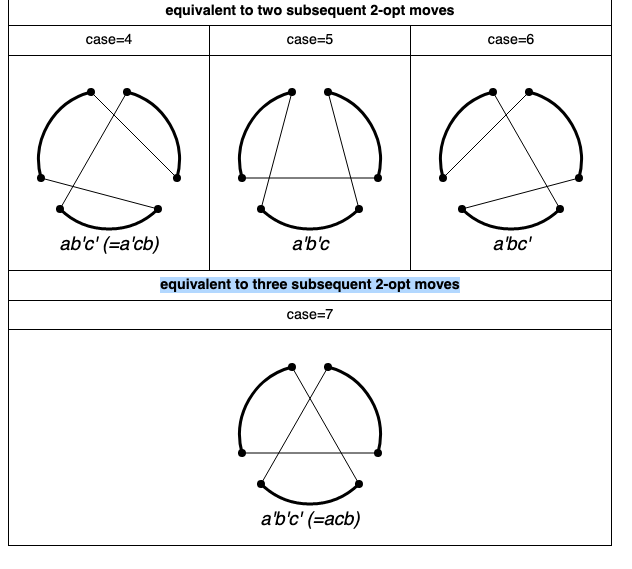
\includegraphics[width=0.4\textwidth]{toDo2}
	\caption{TODO2.}
	\label{toDo2}
\end{figure}

\subsection{Displacement mutation}

This mutation operator \cite{akay2013recent} takes three indices, which define three cut points. The cities which occupy the positions between the first cut point(inclusively) and the second cut point(inclusively) are shifted at the position after the third cut point.  It means that the cities between the second cut point(exclusively) and the third cut point(inclusively) go automatically to the beginning, where the first cut point was. Given the chromosome 0,1,4,5,3,2,7,6 the displacement mutation for the cut points 1, 4 and 6 generates the chromosome 0,2,7,1,4,5,3,6 (see figure \ref{displacement_mutation}).

\begin{figure}[!ht]
	\centering
	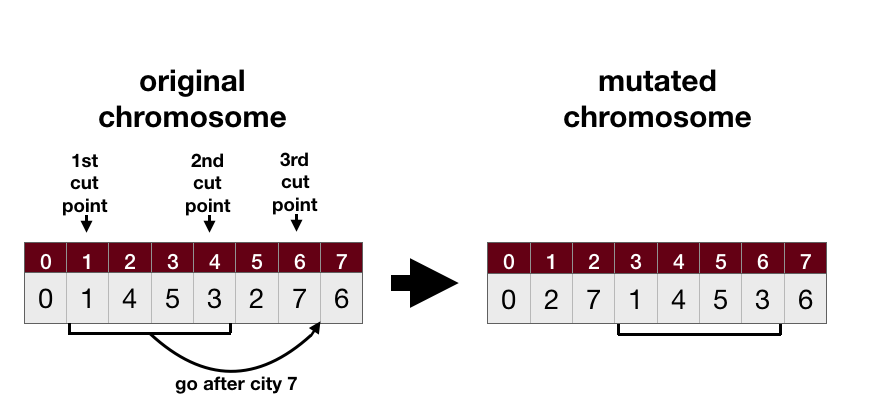
\includegraphics[width=0.5\textwidth]{displacement_mutation}
	\caption{Displacement mutation for the chromosome 0,1,4,5,3,2,7,6 and cut points 1, 4 and 6.}
	\label{displacement_mutation}
\end{figure}

%\subsection{Assigned mutation}
\subsection{Implementation details}

\section{Constructive heuristics}

There are three types of heuristics: constructive, improvement and composite...

This chapter gives an overview of construction heuristics, which will be used for our research. The main goal of construction heuristics is to find solutions in relatively short time. However, the solutions, delivered by them, are not guaranteed to be optimal.  Constructive heuristics build the tour successively and greedy, using some construction rules, without trying to improve the existing part tour. We will use the term "part tour" in the following, meaning the part of the resulting tour, which has been built at the moment.  It means that the part tour, which was already built, remains unchanged. It is important for these heuristics which city will be visited first, because the solutions differ dependent on which starting point is chosen. \par
We will use these heuristics as a starting point for our genetic algorithm, because the first generation of population has to be somehow initialized. We can generate the solutions randomly, but to guarantee that the first generation has at least several "good enough" solutions and not only the random permutations, we will generate them using the following constructive heuristics: nearest neighbor, double-nearest neighbor, nearest insertion, farthest insertion and cheapest insertion.

\subsection{Nearest Neighbor}

The nearest-neighbor (NN) heuristic is a greedy construction heuristic.  Considering a part tour is already built, the NN  looks for a city, which is closest to the last city of the tour, and insert this new found city at the end of the tour.
The algorithm includes the following steps:
\begin{enumerate}
	\item Choose an arbitrary city $s$ as a starting point of the tour.
	\item  Find a city $k$, which is nearest to the city $s$ and add it to the tour right after the city $s$.
	\item Repeat step 2 until the tour includes all the cities to be visited.
	\item Join the last city to the first one, so that we have a cycle.
\end{enumerate}

\subsection{Double Nearest Neighbor}
The double-nearest-neighbor (DNN) heuristic is a modified version of the NN. Considering the part tour is already built, The DNN looks for a neighbor, which is closest either to the first city of the existing part tour or the last one. The found neighbor willl be inserted before the first city of the tour in the first case and after the last city in the second case.
The DNN algorithm includes the following steps:

\begin{enumerate}
	\item Choose an arbitrary city $s$ as a starting point of the tour.
	\item  Find a city $k$, which is nearest to the city $s$ and add it to the tour right after the city $s$.
	\item  Find a city $i$, which is nearest to the city of the tour $s$ or the lat city of the tour 
	\item  Add the city $i$ to the tour right before the city $s$.
	\item Repeat step 2 until the tour includes all the cities to be visited.
	\item Join the last city to the first one, so that we have a cycle.
\end{enumerate}
\subsection{Nearest Insertion}

The nearest-insertion algorithm(NI) includes the following steps:
\begin{enumerate}
	\item Choose an arbitrary city $s$ as a starting point of the tour.
	\item Find a city, which is the nearest to the city $s$ and add it to the tour right after the city $s$.
	\item For each not used city $i$ find its distance to the part touri which s defined as $d(i, T) = \min _{c \notin T}d(c, T)$. It means that the distance to the part tour corresponds to the distance to the city $c$ in the tour which is at nearest to the city $i$
	\item After that, choose the city $j$ amoung all these unused cities, which has with the smallest distance to the part tour.
	\item Find a pair of cities, which are in the tour, between which the city k will be inserted, so that
	the insertion costs are the minimal.
	\item Insert the city k between the cities of the found pair.
	\item Go to the step 3 until the tour includes all the cities to be visited, i.e. there appears the Hamilton cycle.
\end{enumerate}


\subsection{Farthest Insertion}
The farthest insertion-insertion(FI) heuristic repeats the NI algorithm except the step 4, where it chooses the city among the list of unused cities, which has the largest distance to the part tour. 

\subsection{Cheapest Insertion}
\subsection{Implementation details}



\section{Experiments}

\subsection{Definition of general parameters for genetic algorithms}
\subsubsection{Methods}
\subsubsection{Results and discussion}
Sensitivity study

Determining general parameters for a genetic algorithm  influences the quality of the solutions which are produced. 

Population size. 
The choice of an adequate population size for a chosen domain can be problematic. On the one hand, if the size of the population is set too small, it is hard for the genetic algorithm to find good solutions, namely the chromosomes with a good fitness value. On the other hand, too large size can cause very high processing time and very slow convergence. 

\subsection{Combination of mutation and crossover operators}
\subsubsection{Methods}
\subsubsection{Results and discussion}

\subsection{Comparison of effectiveness of different representation types}
\subsubsection{Methods}
\subsubsection{Results and discussion}

\subsection{General discussion}

\section{Conclusion}




\newpage

% Literaturliste soll im Inhaltsverzeichnis auftauchen
\newpage
\addcontentsline{toc}{section}{Literatur}

\bibliography{literatur}
\bibliographystyle{plain}


\end{document}